\chapter[Coalitions and Separation of Powers]{RAW, Eric Temple Bell, the Law of Fives, Coalitions and Separation of Powers}
\chapterauthor{Griffensteed the 5$^\text{lth}$}

\blockquote{
\small{``What Weishaupt discovered that night of February second, seventeen seventy-six,'' Hagbard Celine explained to Joe Malik in 1973, on a clear autumn day in Miami, about the same time that Captain Tequilla y Mota was reading Luttwak on the coup d'\'etat and making his first moves toward the officer's cabal that later seized Fernando Poo, ``was basically a simple mathematical relationship. It's so simple, in fact, that most administrators and bureaucrats never notice it. lust as the householder doesn't notice the humble termite, until it's too late. . . . Here, take this paper and figure for yourself. How many permutations are there in a system of four elements?''

Joe, recalling his high school math, wrote $4\times3\times2\times1$, and read aloud his answer ``Twenty-four.''

``And if you're one of-the elements, the number of coalitions --- or to be sinister, conspiracies --- that you may have to confront would be twenty-three. Despite Simon Moon's obsessions, the twenty-three has no particularly mystic significance,'' Hagbard added quickly. ``Just consider it pragmatically --- it's a number of possible relationships which the brain can remember 	and handle. But now suppose the system has five elements . . . ?.''

Joe wrote $5\times4\times3\times2\times1$ and read aloud, ``One hundred and twenty.''

``You see? One always encounters jumps of that size when dealing with permutations and combinations. But, as I say, administrators as a rule aren't aware of this. Korzybski pointed out, back in the early thirties, that nobody should ever \textit{directly} supervise more than four subordinates, because the twenty-four possible coalitions ordinary office politics can create are enough to tax any brain. When it jumps up to one hundred and twenty, the administrator is lost. That, in essence, is the sociological aspect of the mysterious Law of Fives. The Illuminati always has five leaders in each nation, and five international Illuminati Primi supervising all of them, but each runs his own show more of less independent of the other four, united only by their common commitment to the Goal of Gruad.'' Hagbard paused to relight his long, black Italian cigar.}
\par\begin{flushright} \textup{--- Robert Shea \& Robert Anton Wilson}, Illuminatus!, 1975. \end{flushright}
}

\begin{center}

\includegraphics[scale=0.1]{./img/eris.png}
\end{center}

\section*{Combinatorics of coalitions}
Contrary to what is explained by Hagbard Celine in the introductory excerpt, the number of coalitions --- or to be sinister, conspiracies --- that you can obtain with a system of $n$ elements is not related to the number of permutations but is rather related to the problem of partition of a set; another problem from combinatorics with a more complex mathematical relationship.\\

On the one hand, the number of permutations of $n$ elements corresponds to the number of ways to arrange the $n$ elements in a row \cite{Graham1988}. For instance, for the set $\{1,2,3\}$ there are six possible permutations:
\begin{gather*}
(1,2,3) \qquad (1,3,2) \qquad (2,1,3) \\ 
(2,3,1) \qquad (3,1,2) \qquad (3,2,1)
\end{gather*}
In this case, Joe Malik did the correct computation when it came to permutations, as instructed by Hagbard. There are $n$ choices for the first element, $n-1$ choices for the second, $n-2$ for the third, and so on, giving $n\times(n-1)\times(n-2)\times...\times1$, i.e.
\begin{equation}
n! = \prod\limits_{k = 1}^n k
\end{equation}
The integer sequence of factorial numbers (starting with $0!$) is: $1, 1, 2, 6, 24, 120, 720, ...$ (sequence A000142 on the On-Line Encyclopedia of Integer Sequences\footnote{\url{https://oeis.org}}).
However, permutations only show ways of arranging elements but do not deal with the different way of grouping together the different elements and therefore are not a good model for coalitions.\\

On the other hand, a partition of a set $S$ of $n$ elements is a family of disjoint subsets of $S$ called ``blocks'' whose union is $S$ \cite{Rota1964}.
In other words, it corresponds to a way of grouping all the elements of the set in subsets, i.e. the different coalitions possible with $n$ elements. For instance, for the set $\{1,2,3\}$, there are five possible partitions:
\begin{gather*}
(\{1\},\{2\},\{3\}) \quad (\{1,2\},\{3\}) \quad (\{1,3\},\{2\}) \\
(\{1\},\{2,3\}) \quad  (\{1,2,3\})
\end{gather*}
Counting the number of partitions of a set with $n$ elements is a bit more complicated. It corresponds to the Bell number $B_n$, named after Eric Temple Bell, that can be computed with the following recursive formula:

\begin{equation}
    \begin{cases}
         B_0 = 1\\
         B_{n+1} = \sum\limits_{k=0}^n \binom nk B_k \quad \text{.}
     \end{cases}
\end{equation}
The demonstration for this formula and other formulae for Bell numbers can be found in \cite{Graham1988, Rota1964}.
Another method to compute Bell numbers is to construct the Bell triangle \cite{Aitken1933}. This triangle is constructed by following these rules:
\begin{itemize}
\item start with the number 1,
\item for each new row, the leftmost value is a copy of the rightmost value of the previous row,
\item all the other values are the sum of the value at its left and upper left.
\end{itemize}
 The first few rows of the Bell triangle are shown in Figure \ref{bell}. The integer sequence of Bell numbers (starting from $B_0$) is: $1, 1, 2, 5, 15, 52, 203, ...$ (sequence A000110 on the OEIS).\\

\begin{figure}[h]
\begin{center}
 \[ 
    \begin{matrix}
    1 & & & & & & & \longrightarrow & B_1= 1\\
    1 & 2 & & & & & & \longrightarrow & B_2= 2\\
    2 & 3 & 5 & & & & & \longrightarrow & B_3= 5\\
    5 & 7 & 10 & 15 & & &&  \longrightarrow & B_4= 15\\
    15 & 20 & 27 & 37 & 52 & & & \longrightarrow & B_5= 52\\
    52 & 67 & 87 & 114 & 151 & 203 & & \longrightarrow & B_6= 203\\    
    \vdots\\
    \end{matrix}
\]
\caption{\label{bell} First rows of the Bell Triangle}
\end{center}
\end{figure}

Things get even more complicated if we consider that the partitions can be ordered. In this case, the different permutations of a given partition have to be considered. This is called weak ordering and can be used to determine the number of ways of ordering $n$ players when ties are possible \cite{Good1975}. In our case, it can be used to represent the unbalanced power relationships between the different elements/coalitions. For instance, for the set $\{1,2,3\}$, there are thirteen possible \emph{ordered partitions}:
\begin{gather*}
(\{1\},\{2\},\{3\}) \quad (\{1\},\{3\},\{2\}) \\ 
(\{2\},\{1\},\{3\}) \quad (\{2\},\{3\},\{1\}) \\ 
(\{3\},\{1\},\{2\}) \quad (\{3\},\{2\},\{1\}) \\
(\{1\},\{2,3\}) \quad (\{2,3\},\{1\}) \quad (\{2\},\{1,3\}) \\
(\{1,3\},\{2\}) \quad (\{3\},\{1,2\}) \quad (\{1,2\},\{3\}) \\
(\{1,2,3\})
\end{gather*}
The number of possible ordered partitions of a set of $n$ elements is given by the ordered Bell numbers (also called Fubini numbers), defined by \cite{Knuth1998}:
\begin{equation}
     a_n= \sum\limits_{k=0}^n k! \;  S(n,k) \quad \text{,}
\end{equation}
where $S(n,k)$ is the Stirling number of the second kind, corresponding to the number of ways to partition a set of $n$ objects into $k$ non-empty subsets, that can be computed with the recursive formula \cite{Graham1988}:
\begin{equation}
    \begin{cases}
    S(0,0) = 1 \quad \text{and} \quad S(0,n) = S(n,0) = 0\\
    S(n+1,k) = kS(n,k) + S(n,k-1)
    \end{cases}
\end{equation}
The integer sequence of ordered Bell numbers (starting from $a_0$) is: $1, 1, 3, 13, 75, 541, 4683,  ...$ (sequence A000670 on the OEIS).

\section*{The implications}

Back to our coalitions --- or to be sinister, conspiracies --- and to the excerpt from \textit{Illuminatus!} If we first consider non-ordered partitions: ``How many different partitions are there in a system of four elements?'', should have asked Hagbard Celine.\\
Joe wrote the beginning of the sequence of Bell numbers and read aloud ``the fourth Bell number is fifteen.''\\
So, if you remove the state where all the elements are separated, that is without any coalition, it means that the number of possible coalitions with four elements you may have to confront would be fourteen\footnote{$1+4=5$, but let us forget about the magick of the Law of Fives \cite{Malaclypse1963}.}. But now, what about a system of five elements?\\
Joe read aloud ``the fifth Bell number is fifty-two.''\\
Analogously, the number of possible coalitions with four elements you may have to confront would be fifty-one. Figure \ref{part} shows the 52 different partitions of a set of 5 elements.
In this case, even if the problem was not correctly addressed by using permutations instead of partitions, RAW and Korzybski's deduction still stands. 
The jump from fourteen to fifty-one possible relationships is enough to go from something taxing for the brain to something large enough to completly lose it \cite{Kelly1955, Korzybski1933}. \\

\begin{figure}
\begin{center}
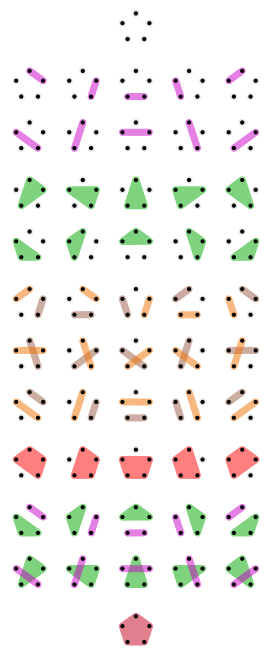
\includegraphics[scale=0.7]{./img/part.png}
\caption{\label{part} The 52 partitions of a set of 5 elements (source: wikipedia)}
\end{center}
\end{figure}

Now, if we consider ordered partitions, the jump appears earlier. The third ordered Bell number is thirteen and the fourth ordered Bell number is seventy-five\footnote{$75=5\times 15$ }. Moreover, in this case, all configurations are problematic, since they represent either coalitions or unbalanced power relations between elements. With this model, RAW and Korzybski's deduction appears earlier than they formulated it in term of number elements; four elements becoming the new tipping point.


\section*{The Law of Fives and the separation of powers}

When expressing the necessary bases for true democracy, John Locke and Montesquieu identify the need for the separation of powers (i.e. absence of coalition between powers) for \textit{representative democracy} in their respective essays \textit{Two Treatises of Government} \cite{Locke1689} and \textit{De l'esprit des lois} \cite{Montesquieu1748}. Moreover, modern criticisms of their work, when it comes to establish democracy, are aimed first at the fact that the organizations proposed respectively by Locke and Montesquieu do not provide a real separation of the powers but rather an interlocking of the powers; and second at the fact that the different powers identified are not put on an equal footing, some being more important than others.\\

Montesquieu identifies three powers \cite{Montesquieu1748}, that are now represented by different institutions in many representative democracies following the \textit{Age of Enlightenment}:
\begin{itemize}
\item the legislative power,
\item the executive power,
\item the judicial power.
\end{itemize}
In this setting with three powers, the third Bell number tells us that the number of possible coalitions (and therefore absence of true separation of powers) is four ($B_3 - 1$), and the third ordered Bell number tells us that number of possible coalitions or unbalanced power relations (and therefore absence of true separation of powers or equality between powers) is thirteen ($a_3$).\\
In other words, with both models, we obtain a number of possible relationships which the brain, the institutions, and people can handle.
It would therefore be theoretically possible to obtain true democracy with representative democracy.\\

However, new powers have been identified since, in particular:
\begin{itemize}
\item the mediatic power (also called ``the fourth power'') \cite{Bourdieu1996, Herman1988},
\item the economic power (also called ``the fifth power'') \cite{Ramonet1989, Ramonet1996}.
\end{itemize}
Adding these two powers changes the setting drastically. Having five powers means that the number of possible coalitions is given by the fifth Bell number, that is to say fifty-one ($B_5 -1$), and the number of possible coalitions or unbalanced power relations is five hundred and forty-one ($a_5$).\\
This situation becomes alarming because on top of not having institutions to help the separation of these new powers with the others (since the institutions have been created before their identification), the number of possible coalitions and unbalanced power relations becomes way too taxing for the brain, the institutions, and people to handle. Moreover, this issue can only get much worse the more powers are identified (we could, for instance, add Internet and public opinion\footnote{$B_6 = 203$ and $a_6 = 4683$.}) with jumps always getting larger.\\

\section*{Conclusion}

For these reasons, I would conclude that separation of powers is not enough of a base for true democracy. Consequently, representative democracies are not a viable political systems since it can not prevent a reign of power(s) and only encourages new aristocracies of greyfaces and totalitarianism. 
I would therefore encourage members of \textsc{The House of the Rising Collapse} to launch an \textit{Erisian Movement for Dysnomia, Daughter of Goddess} with a main focus on a total dissolution of all form of power and a direct democracy.

\begin{center}
\textit{Don't let them immanentize the eschaton!\\}


\includegraphics[scale=0.3]{./img/poee.png}
\end{center}

\section*{Acknowledgements}
This article has been written for the Patafizikhood of Eris Esoteric. It has NOT been conducted with the support of the AISB. Consult your pineal gland. \textsc{All Hail Discordia!!!!!}

%References
\bibliographystyle{unsrt}
\bibliography{coalitions_biblio}